
\documentclass[10pt]{article}
%	options include 12pt or 11pt or 10pt
%	classes include article, report, book, letter, thesis

\usepackage[a4paper,bindingoffset=0.2in,%
            left=1in,right=1in,top=0.2in,bottom=0.3in,%
            footskip=.15in]{geometry}
            
\usepackage[T1]{fontenc}
\usepackage[polish]{babel}
\usepackage[utf8]{inputenc}
\usepackage{lmodern}
\selectlanguage{polish}
\usepackage{blindtext}
\usepackage{pgfplots}
\usepackage{graphicx}

\title{Algorytmy numeryczne}
\author{Zadanie 1 \\ Aleksander Kosma\\grupa 1 tester-programista}
\date{16 Październik 2017}

\begin{document}
\maketitle 

\section{Sumowanie szeregów potęgowych}



Opracowanie prezentuje próby obliczenia funkcji arctan, przy pomocy języka java.
Wykorzystano w tym celu dwa sposoby na obliczenie tej wartości. Są to:\\
-zsumowanie elementów wyliczonych z szeregu potęgowego:\\
$$arctg(x) = \sum_{n=0}^{\infty}\frac{(-1)^n}{2n + 1} x^{2n + 1}$$
-zsumowanie elementów wyliczonych na podstawie poprzednika:\\
$$a_{n+1}= a *-\frac{x^2 * (2n + 1)}{2n + 3}$$

Ze względu na charakter obliczeń podzieliłem owe zsumowania na kolejne dwa:\\
-zsumowanie elementów licząc od tyłu\\
-zsumowanie elementów licząc od przodu\\

Wnioski zostały obliczone na zmiennej typu double. Również ze względu na zbieżność szeregu w $[-1,1]$ 
liczyłem tylko dla tego zakresu.\\

Wykres przedstawia który rodzaj sumowania ma większą szanse na precyzyjniejszy wynik względem drugiego.
Każda kolumna wartości została wyliczona dla 100 tysięcy liczb między podanymi przedziałami. Razem 2 miliony próbek.\\


\begin{center}
 \makebox[\textwidth]{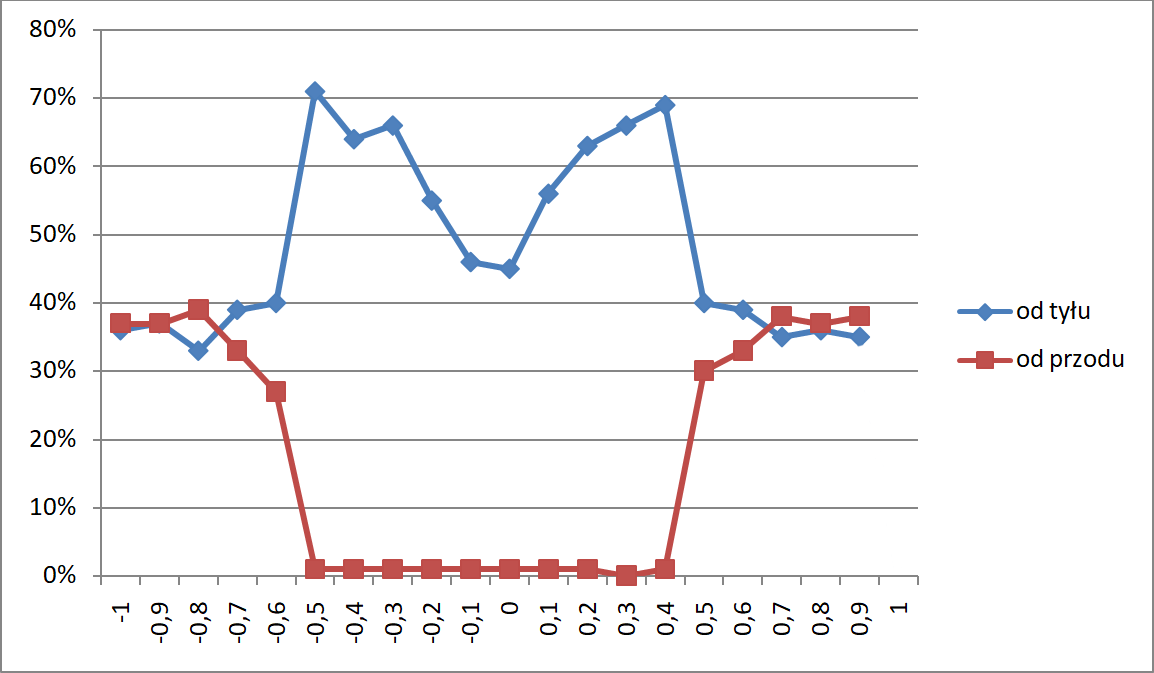
\includegraphics[width=0.7\paperwidth]{rozklad_procentowy.png}}
\end{center}


Drugi wykres prezentuje bezwzględną różnice między wynikiem biblioteki a sumowaniami. Można zauważyć, że przez większą część spektrum wartości, sumowanie tylne jest precyzyjniejsze nawet o 2 rzędy wielkości.


\begin{center}
 \makebox[\textwidth]{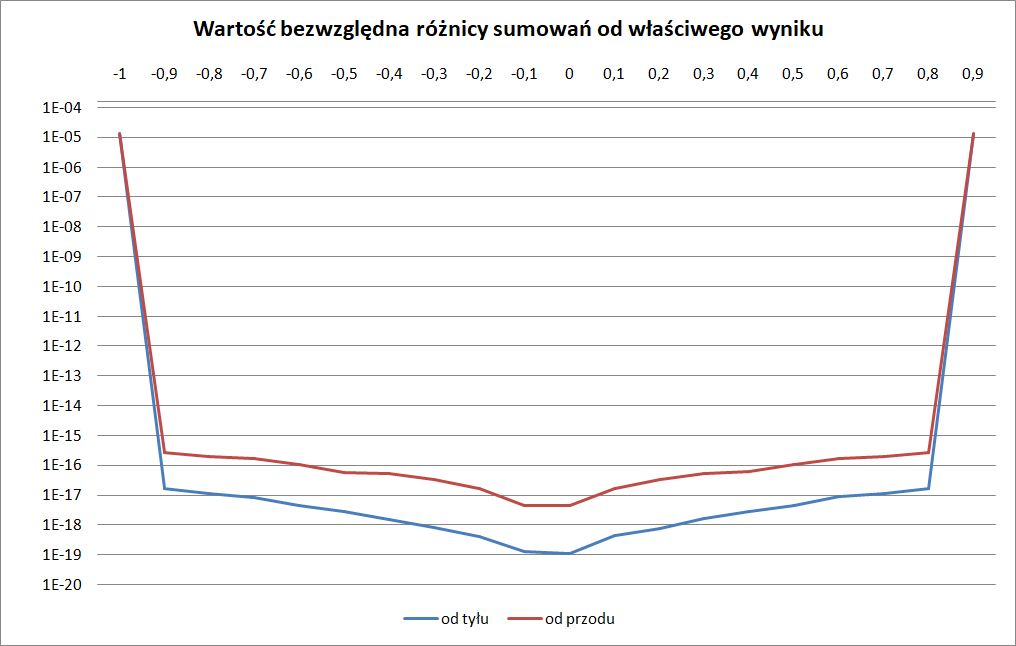
\includegraphics[width=0.65\paperwidth]{rozklad.png}}
\end{center}

Takie rezultaty wynikają z natury działania zmiennej double. W przypadku sumowania liczby większej do liczby mniejszej(gdzie różnica wynosi parę rzędów wielkości), zmienna odrzuca końcowe cyfry mniejszej liczby by pomieścić najistotniejsze wartości. Stąd utrata precyzji. W momencie kiedy dwie liczby mają podobną wartość, ich suma potrzebować będzie podobnej precyzji do zapisania wyniku. W konsekwencji nie odrzuci danych. Podsumowując kwestie precyzji wyniku. Opierając się o zmienną double, można stwierdzić, że precyzja wyniku waha się między 14, a 16 miejscem po przecinku.\\
Na obrazku poniżej znajduje się praktyczny przykład. Dla uproszczenia zagadnienia jest on prezentowany na zmiennej float(32 bity) która zazwyczaj mieści w sobie 8 cyfr dziesiętnych.\\

\begin{center}
 \makebox[\textwidth]{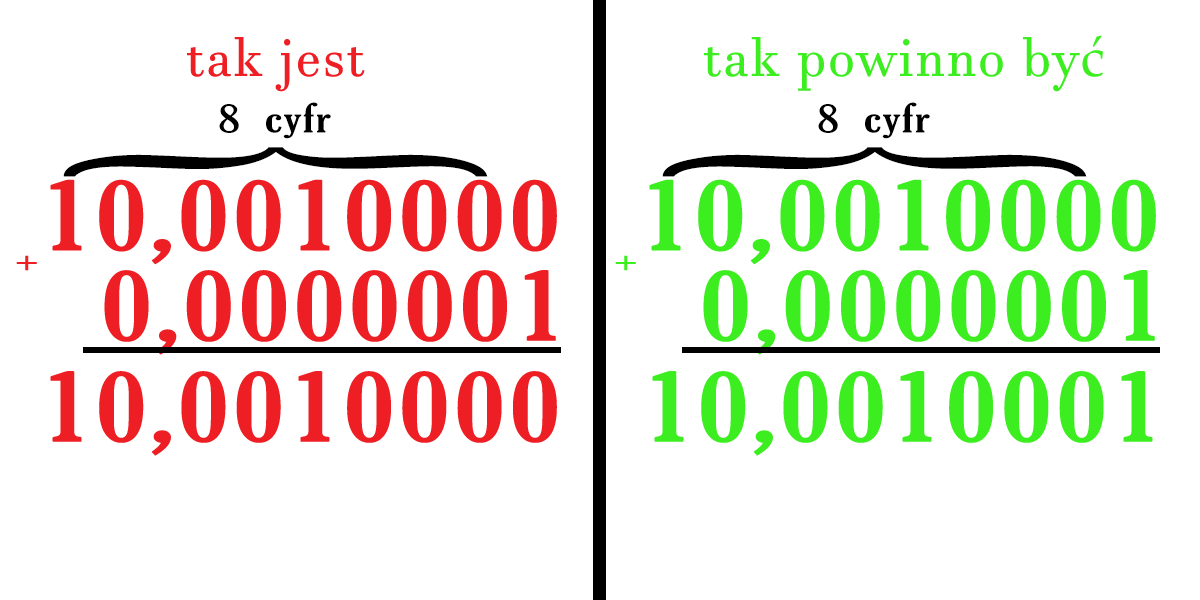
\includegraphics[width=0.4\paperwidth]{przyklad.png}}
\end{center}

By rozwiązać problem niskiej precyzji, który zaistniał w przypadku doubla, trzeba mieć kontrolę nad precyzją obliczeń. Rozwiązaniem może okazać się klasa BigDecimal. Klasa ta może przechować nieograniczoną 
wartość liczbową, ogranicza ją jedynie skala która osiąga wartość 32-bitowego integera, czyli trochę 
ponad dwa miliardy miejsc. \\
Udało mi się osiągnąć praktycznie nieograniczoną precyzję. Wyniki oparte o BigDecimal porównywałem z kalkulatorem online Wolfram(computational knowledge engine). Przykładowy wypis programu wraz ze wszystkimi rodzajami obliczeń i ich wynikami. W tym przypadku podana precyzja BigDecimal i Wolfram to 64 miejsca po przecinku.

\begin{center}
 \makebox[\textwidth]{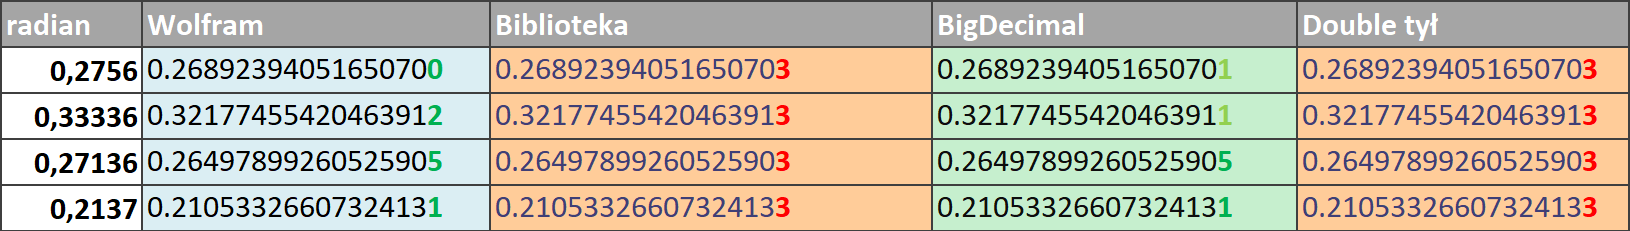
\includegraphics[width=0.8\paperwidth]{bigDecimal.png}}
\end{center}









\end{document}